\section*{Spécifications matérielles}

\begin{table}

\label{my-label}

\begin{tabular}{l|p{90mm}}
\hline
\rowcolor[HTML]{FFFFFF} 
\multicolumn{2}{c}{\cellcolor[HTML]{FFFFFF}\textbf{SARA}}                                                      \\ \hline
\rowcolor[HTML]{EAEFF6} 
\textbf{Base}               & Base avec roues holonomiques mecanums \\
\rowcolor[HTML]{FFFFFF} 
\textbf{Bras}          & 7 DoF custom arm made of Kinova motors                                           \\
\rowcolor[HTML]{EAEFF6} 
\textbf{Cou}               & Tilt and pan unit using two Dynamixel MX-64R servo actuator                      \\
\rowcolor[HTML]{FFFFFF} 
\textbf{Tête}               & Custom head made of RGB neopixels leds and Asus Xtion Pro                        \\
\rowcolor[HTML]{EAEFF6} 
\textbf{Pince robotique}            & Robotiq 2 doigts 140mm                                                           \\
\rowcolor[HTML]{FFFFFF}
\textbf{Dimensions}         & \begin{tabular}[c]{@{}l@{}}Base : 0,61m. X 0,77m.\\ Height : 1,68m.\end{tabular} \\
\rowcolor[HTML]{EAEFF6} 
\textbf{Poids}             & $\sim$60kg                                                                      \\
\rowcolor[HTML]{FFFFFF} 
\textbf{Capteurs additionnels} & Hokuyo UTM-30LX on base                                                          \\
\rowcolor[HTML]{EAEFF6} 
\textbf{Microphone}         & Microphone Rode											                         \\
\rowcolor[HTML]{FFFFFF} 
\textbf{Batteries}          & 2x 20V Dewalt drill batteries 5aH                                                 \\
\rowcolor[HTML]{EAEFF6} 
\textbf{Ordinateur}           & 1x Lenovo p50 avec 32GB RAM et nVidia Quadro M2000 4GB, 1x Raspberry Pi 3       \\ \hline
\end{tabular}
\caption{Robot's hardware description}
\end{table}
\begin{wrapfigure}[10]{r}{0.25\textwidth}
	\centering
	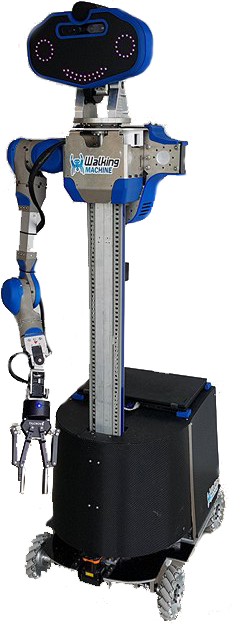
\includegraphics[width=0.30\textwidth]{images/sara_2.png}
	\caption{Robot SARA}
\end{wrapfigure}
\section*{Robot's Software Description}

For our robot we are using the following software:

\begin{itemize}
	\item Platform: Robotic Operating System (ROS) Kinetic on Ubuntu 16.04
	\item Navigation, localization and mapping: \href{http://wiki.ros.org/gmapping}{Gmapping}, \href{http://wiki.ros.org/amcl}{AMCL}, \href{http://wiki.ros.org/pointcloud_to_laserscan}{pointcloud\_to\_laserscan}
	\item Face recognition: \href{http://wiki.ros.org/people}{People}
	\item Speech recognition: \href{https://github.com/WalkingMachine/lab_ros_speech_to_text}{Google Speech API}
	\item Speech comprehension: \href{http://sag.art.uniroma2.it/lu4r.html}{LU4R}, \href{https://github.com/WalkingMachine/lu4r_ros}{lu4r\_ros}
	\item Speech generation: \href{https://doc.ubuntu-fr.org/svoxpico}{Svoxpico}
	\item Object recognition: \href{https://github.com/WalkingMachine/wm_darknet}{Darknet with YOLO v2 }
	\item Arm control: \href{http://wiki.ros.org/moveit}{MoveIt} and \href{https://github.com/Kinovarobotics/kinova-ros}{Kinova API}
	\item Task executor: \href{http://wiki.ros.org/flexbe}{Flexbe} 
	\item World reprensentation: \href{http://github.com/walkingmachine/wonderland}{Wonderland}
\end{itemize}